% Subsection: time-dependent travel times (\input from sections/sequential.tex)
\subsection{Time-dependent travel times (the lecturer's model)}
\label{sec:seq-td}

The reference notebook makes $h$ dynamic in a concrete way: the speed changes
with the time of day. A profile of 20 slots gives one network-wide speed per
slot (350--600\,m/min), and a trip that departs at time $t$ drives at
$\mathit{speeds}[\lfloor t \rfloor]$. Both the travel time of an edge and the
heuristic then depend on the time at which a node is reached. We implemented
this model in C++ (\texttt{td\_astar}, \texttt{SpeedProfile}) with three
corrections to the notebook (Section~\ref{sec:review}):

\begin{enumerate}[nosep]
  \item \textbf{FIFO edge times.} The time to drive an edge integrates the
        speed over every slot the edge spans. Leaving later can then never
        mean arriving earlier, which is the condition under which
        label-setting A* (and Dijkstra) remain exact for time-dependent costs.
        Using only the speed at departure, as the notebook does, violates this
        for 6.3\% of random (departure time, length) pairs.
  \item \textbf{Admissible heuristic.} $h(v) = d_{\mathrm{gc}}(v,t)/v_{\max}$,
        where $d_{\mathrm{gc}}$ is the great-circle distance and $v_{\max}$ the
        highest speed of the profile, never over-estimates, whatever the time.
        The notebook divides by the speed at the current time, which
        over-estimates whenever faster slots follow.
  \item \textbf{Cyclic profile,} so that trips longer than 20 slots stay
        inside the array.
\end{enumerate}

\paragraph{Testing.} Test T6 checks FIFO on 200\,000 random pairs, and runs
100 random queries at random departure times. Because the speed is the same on
every road at a given moment and travel is FIFO, the fastest route is the
shortest-length route, and its travel time is $\mathrm{arrive}(t_0, L^*) - t_0$.
This gives an oracle that does not share code with A*. Time-dependent A* and
time-dependent Dijkstra must both match it to $10^{-6}$\,min; they do on all
five platforms.

\begin{table}[H]
\centering
\small
\caption{Part 1: time-dependent A* with the lecturer's speed profile; 200
queries $\times$ 4 departure times. Expanded, re-opened and quality
(cost/optimum) are from Platform~C; B and C use the same queries. The road
distance $d_{\mathrm{road}}$ needs one reverse Dijkstra per destination, which
is not included in the time.}
\label{tab:td}
\begin{tabular}{l rrrrr r}
\toprule
Heuristic & ms (A) & ms (C) & expanded & re-opened & mean & worst \\
\midrule
$h = 0$ (time-dependent Dijkstra) & 6.6 & 19.8 & 104{,}414 & 0 & 1.000 & 1.000 \\
$h = d_{\mathrm{gc}} / v_{\max}$ & 4.3 & 12.8 & 44{,}367 & 0 & 1.000 & 1.000 \\
$h = d_{\mathrm{road}} / v_{\max}$ (one reverse Dijkstra) & 2.0 & 5.7 & 25{,}439 & 0 & 1.000 & 1.000 \\
$h = d_{\mathrm{gc}} / \mathit{speed}(t)$ (lecturer) & 4.5 & 16.2 & 62{,}804 & 45{,}665 & 1.045 & 1.288 \\
\bottomrule
\end{tabular}

\end{table}

\begin{figure}[H]
\centering
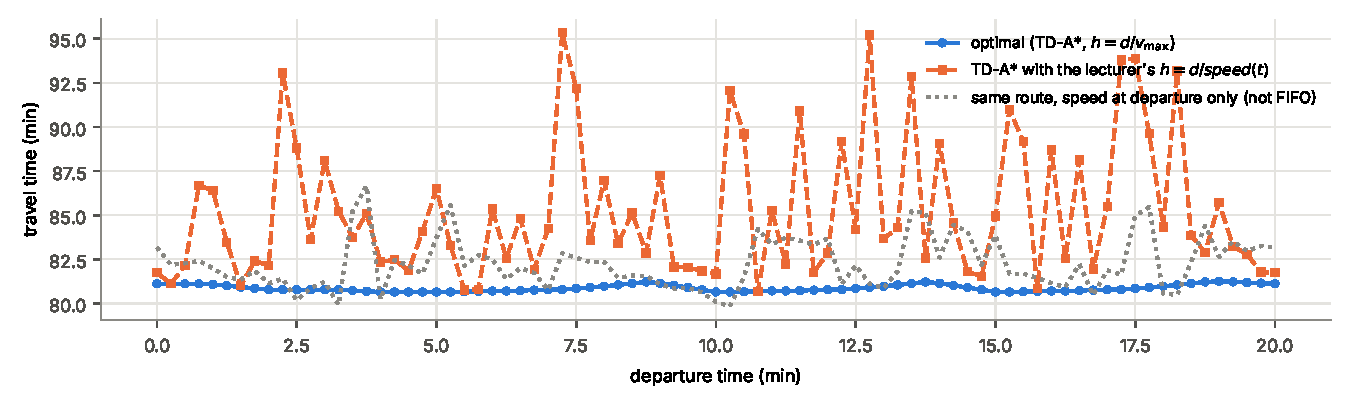
\includegraphics[width=\linewidth]{figures/fig9_td.pdf}
\caption{Part 1: travel time of the longest of the 200 queries as a function
of the departure time (Platform~C).}
\label{fig:td}
\end{figure}

\textbf{The lecturer's heuristic is not admissible, and it shows.} With
$h = d/\mathit{speed}(t)$, 87\% of the 800 runs return a route that is slower
than the optimum, by 4.5\% on average and by up to 29\%. Because the
estimate jumps whenever the clock crosses a slot boundary, the search also
re-opens 45\,665 nodes per query. It is not even faster: it expands more nodes
than the admissible great-circle heuristic (62\,804 against 44\,367).
Figure~\ref{fig:td} shows the same effect for one long trip: the optimal
travel time varies by only 0.6\,min with the departure time, while the
lecturer's heuristic adds up to 14.5\,min. The non-FIFO edge model of the
notebook gives yet another travel time, between 0.9\,min less and 6.0\,min more than the
correct one, because it charges the whole edge at the speed of the slot in which the
car enters it.

\textbf{A better admissible heuristic pays off.} The road distance to the
target divided by $v_{\max}$ is still admissible but much tighter: it needs
43\% fewer expansions than the great-circle heuristic (25\,439 against 44\,367) and is
3.3--3.5$\times$ faster than time-dependent Dijkstra. This is the correct version
of the notebook's \texttt{shortest\_path\_at\_time} idea: compute the road
distances once per destination with a reverse Dijkstra, instead of one full
search per evaluation of $h$.
